\documentclass[12pt]{article}
\usepackage{ametsoc}
\usepackage{amsmath}
\usepackage[pdftex]{epsfig}
\usepackage{amsfonts}
\usepackage{amssymb}
\include{graphicsx}
\usepackage{lineno}
\linenumbers

\setlength{\textwidth}{6.5in} % 6in
\setlength{\oddsidemargin}{0in}
\renewcommand{\labelenumi}{\arabic{enumi}. }

\begin{document}
\title{Improved Nowcasts By Blending Extrapolation and Model Forecasts}

\author{Yunsung Hwang$^{1, 2, 3}$\thanks{$^1$ Cooperative Institute of Mesoscale Meteorological Studies, University of Oklahoma $^2$ National Severe Storms Laboratory, Norman, OK  $^3$ School of Meteorology, University of Oklahoma}}
%\author{Yunsung Hwang$^{1, 2, 3}$\thanks{Corresponding author: Yunsung Hwang, University of Oklahoma, Norman, OK, yunsung.hwang@ou.edu $^1$ Cooperative Institute of Mesoscale Meteorological Studies, University of Oklahoma $^2$ National Severe Storms Laboratory, Norman, OK  $^3$ School of Meteorology, University of Oklahoma $^4$ Climate Corporation, Seattle, WA },\\  Adam J. Clark$^{1, 2}$, \\ Valliappa Lakshmanan$^{4}$,\\ Steven E. Koch$^{2, 3}$}

\amstitle
%
%\begin{abstract}
%No abstract needed now so comment them
%\end{abstract}

\section{previous studies}

{\color{blue}study of predictability of precipitation from continental radar images in Mcgill}

cite as {maple1method} \citep{maple1method}

cite as {maple2probfcst} \citep{maple2probfcst}

cite as {maple3opr} \citep{maple3opr}

cite as {maple4limit} \citep{maple4limit}

cite as {maple5growthdecay} \citep{maple5growthdecay}






{\color{blue}time-lagged ensemble}

cite as{timelagNWP} \citep{timelagNWP}


\section{Introduction}
 
\section{Data and Methodology}
Add references of mergedQCrelfectivitycomposite and the threshold used to binary decision such as 35 dBZ or 40 dBZ (need ref here).

\subsection{Dataset}
In this study, forecasts and observations of 18 dBZ echo top heights are examined, which are defined as the maximum altitude at which reflectivity exceeds 18 dBZ. The observed echo top heights are estimated from the Weather Surveillance Radar 1988 Doppler (WSR-88D) data using the highest elevation angle that detects reflectivity over 18 dBZ \citep{lak++13}. Echo top heights were chosen for examination because they  are one of the parameters that determine the availability of a flight route in recently developed convective weather avoidance models \citep{mat+10, sheth++13}. For verification purposes, 18 dBZ echo top heights computed from the WSR-88D network covering the Contiguous United States (CONUS) are used as truth. Four different sets of 8 h forecasts are evaluated, which are all initialized at 1800 UTC. This particular initialization time was chosen because it is a few hours before the typical maximum in the diurnal cycle of convection and, thus, precedes by a few hours the largest potential impacts on flight routing. Forecasts on 24 days during the period 15 May to 13 June 2013 were examined (the dates 20, 28, 29 May and 4 and 7 June were excluded because of missing data). The four forecasts consisted of 1) the HRRR model, 2) extrapolated observations, 3) a blending of extrapolated observations and the HRRR referred to as Lin CD, and 4) another blending of extrapolated observations and the HRRR called Sal CD. Details on the four forecasts are discussed in the following sections. 
\subsection{HRRR}
The HRRR model is a convection-allowing model, which generates convection without convective parameterization, covering the Contiguous United States (CONUS) with 3-km grid spacing and is nested within the parent model domain of the 13-km grid-spacing Rapid Refresh (RAP; \citealt{brown++11, wey++11}) model. The RAP provides initial and boundary conditions and assimilates radar reflectivity observations through a diabatic digital filter initialization \citep{huang+93}. The HRRR model is based on the Advanced Research core of the Weather Research and Forecasting (WRF) model (ARW; \citealt{skam++08}) with the following WRF physics options: 
1) Goddard shortwave radiation scheme \citep{chou94}, 
2) Rapid radiative transfer model longwave radiation scheme \citep{mlawer++97}, 
3) RUC Smirnova land surface model \citep{smirnova++97}, 
4) Mellor-Yamada-Nakanishi-Niino (MYNN) boundary layer parameterization \citep{nakanishi04} 
and 5) Thompson mixed-phase microphysics scheme \citep{thompson++08}.

The RAP and HRRR assimilate data hourly using Gridpoint Statistical Interpolation (GSI). The HRRR utilizes 3-km data assimilation to include detailed observational information using GSI. During a preforecast hour, observed radar reflectivities replace latent heating fields for the HRRR at 15 minute intervals. Moreover, at the beginning of the forecast, a 3-km non-variational cloud analysis and hydrometeor analysis using radar reflectivities are used to obtain additional information about rain and snow mixing ratios. 

\subsection{Extrapolated observations }

The high spatial and temporal resolution of weather radar data has enabled the development of several nowcasting techniques based on extrapolation methods \citep{manda++12}. In these methods the movement of storm cells is typically estimated by matching radar echoes between two successive radar images. A storm cell is typically defined as a region of reflectivity that exceeds a threshold (usually 35 or 40 dBZ). Examples of tracking and extrapolation algorithms found in the literature include Continuity Of Tracking Radar Echoes by Correlation (COTREC; \citealt{li95}), which used variational methods \citep{sasaki58, sasaki70} to skillfully predict the movement of storm cells 20 minutes in advance. The Thunderstorm Identification, Tracking, Analysis and Nowcasting (TITAN; \citealt{dixon93}) system was created to optimally match storm cells successive radar images using a linear programming optimization approach called the Hungarian Method. The McGill Algorithm for Precipitation nowcasting method using Lagrangian Extrapolation (MAPLE) \citep{germann02, germann04} applies variational approaches to provide improved extrapolation. 

For extrapolation forecasts, we used the segmotion algorithm that is implemented in the Warning Decision Support System Integrated Information (WDSS-II; \citealt{lak++06}). 
In this technique, thunderstorms are identified at different scales using the extended watershed approach \citep{lak09eff}. The image is ``flooded'' starting from the global maximum. The flooding level is slowly decreased so that flooding can proceed at lower and lower levels and the entire area covered by water flowing from a single maximum to a predetermined size (this size varies by scale) forms a thunderstorm. Storms identified in consecutive images are associated based on a greedy optimization algorithm \citep{lak10object} that tries to optimize the match based on projected storm location and a cost function based on continuity of the maximum value. The motion vector derived from storm associations is interpolated onto the full grid using an inverse distance weighting scheme \citep{lak++03}. These motion vectors, one for each scale, are then matched to the size of the objects being extrapolated and the time period of extrapolation and used to extrapolate the current echo top grid into future time steps.

\subsubsection{Linear cross-dissolve}
Linear cross-dissolve is a commonly-employed blending method that computes the weighted average of two aligned images pixel-by-pixel. For example, if one tries to combine two images $I_{1}$ (the extrapolation) and $I_{2}$ (the model forecast), the cross-dissolve of the images, $C(x,y)$ can be represented as 
\begin{equation}
 C(x,y)=wI_{1}(x,y)+(1-w)I_{2}(x,y)
 \end{equation}
 where $I_{1}(x,y)$ is the intensity of the pixel $(x,y)$ in the first image and $I_{2}(x,y)$ for the second image. Assuming that there are six time steps (0, 1, 2, 3, 4 and 5 h) between $I_{1}$ and $I_{2}$, at 0 h the $C(x,y)$ is the same as $I_{1}$ since $w=1.0$ and $1-w=0.0$. At 3 h,  $C(x,y)=0.6 \times I_{1}(x,y)+0.4 \times I_{2}(x,y)$ gives slightly more weight to $I_{1}$. For morphing extrapolation and model fields, $w$ for a linear cross-dissolve is shown in Fig. \ref{f1}a and $1-w$ Fig. \ref{f1}b. It should be noted that blending weights ($w$) are independent of the intensities $I_{1}(x,y)$ and $I_{2}(x,y)$.
 
 For linear cross-dissolve, the same weights are applied to images at a certain fraction of time for all intensities. Essentially, features from $I_{1}$ fade out as features from $I_{1}$ fade in. Features present in both images fade from their presentation as in $I_{1}$ to their presentation as in $I_{2}$.
 
 Idealized examples of linear cross-dissolve for a line of discrete storm cells are shown in Fig. \ref{f2}. There are six time steps (0, 1, 2, 3, 4 and 5 h) of three convective cells in the illustration. The cells are moving to the east at a constant speed as shown in the first row of Fig. \ref{f2}. The top cell has not developed at 0 h but develops at 1 h and  increases in intensity until 5 h. The center cell decreases in intensity throughout the idealized forecast period while the bottom cell maintains constant intensity. Extrapolation captures only the center and bottom cells from the observation at 0 h and extrapolates them to the east without changing the intensities. The bottom cell is well captured by extrapolation because it is unchanging in time. However, the change in intensity of the center cell is not captured by the extrapolation. On the other hand, it is not possible to extrapolate the top cell since it was not present in the observations at 0 h. In the illustration, it is assumed that the model forecast simulates only the top and the bottom cells, and with lower intensities. 

\section{Discussion and future work}
\subsection{Discussion}

A new technique to blend extrapolation and model forecasts was developed and evaluated using observations and forecasts over 24 days from mid-May to mid-June 2013. In general, blending techniques using weighted averaging apply constant weights for both extrapolation ($w$) and model forecasts ($1-w$) at each forecast lead time. For example, $w$=1.0 is applied to the extrapolation and $1-w$=0.0 is applied to the model forecast at the beginning of the forecast and $w$ decreases gradually to $w$=0.0 at the end of the forecast. The weighted averaging (``Linear cross-dissolve") has a problem producing underestimated blended values during the middle of the forecast, where both $w$ and $1-w$ are close to 0.5 if the forecasts are displaced. To mitigate this problem, the model forecast and extrapolation fields can be aligned before weights are applied, however displacements remain even after this alignment. In order to further improve the blending results, a technique called ``Salient cross-dissolve" is applied in this work. Two-dimensional weights ($w_{s}$) based on the differences between normalized intensities from the extrapolation and model forecast are determined for each forecast hour (as a function of time fraction; $w$). The novelty of salient cross-dissolve is preserving the values either in the extrapolation and model forecasts if they are high enough. For example, if there are two convective cells in both extrapolation and model forecasts in the middle of forecast lead time, salient cross-dissolve tends to shrink the cells by applying different weights (i.e., higher weights are applied to higher values and lower weights are applied to lower values which preserves most of the high-valued pixels and eliminates many of the low-valued pixels) while linear cross-dissolve cuts every value in half. Salient cross-dissolve showed better results than those of linear cross-dissolve in this study. Instead of ``fading out" in linear cross-dissolve, $w_{s}$ enables the pixels with strong intensities to be preserved in salient cross-dissolve resulting in more pixels with higher values. 

For the forecast evaluations, a new method called the route-based segments method, which considers airplane routes, was developed and tested with comparisons made to a neighborhood-based method. Both methods gave very similar results indicating superior performance for the forecasts using Salient cross-dissolve, particularly during forecast hours 2 - 5 h.

%%%==========================================================================
\subsection{Future work}
The contribution of the work is adding additional information to the weights applied to the extrapolations and the model forecasts. Considering differences of normalized intensities showed promising results and helped give more realistic intensities in blended forecasts. Instead of adjusting values in model forecasts based on linear weights that vary as a function of time, salient cross-dissolve also considers intensities so that pixels with high values are retained. However, updated weights, $w_{s}$, do not reflect actual data from the extrapolation nor model forecasts. Future study should consider the processes of adjusting those weights considering the real data and past performance. Additionally, frequently updating extrapolation, in other words, adding latest observational information at 15 minute time intervals should be utilized. Finally, it is also possible to consider weights as two separate variables instead of using $w_{s}$ and $1-w_{s}$. The independent variables can be adjusted using machine learning. Updated techniques using such methods are planned for future applications.  




%------------------------------------------------------------Fig.s
%\begin{figure}[t]
%\begin{center}
%\noindent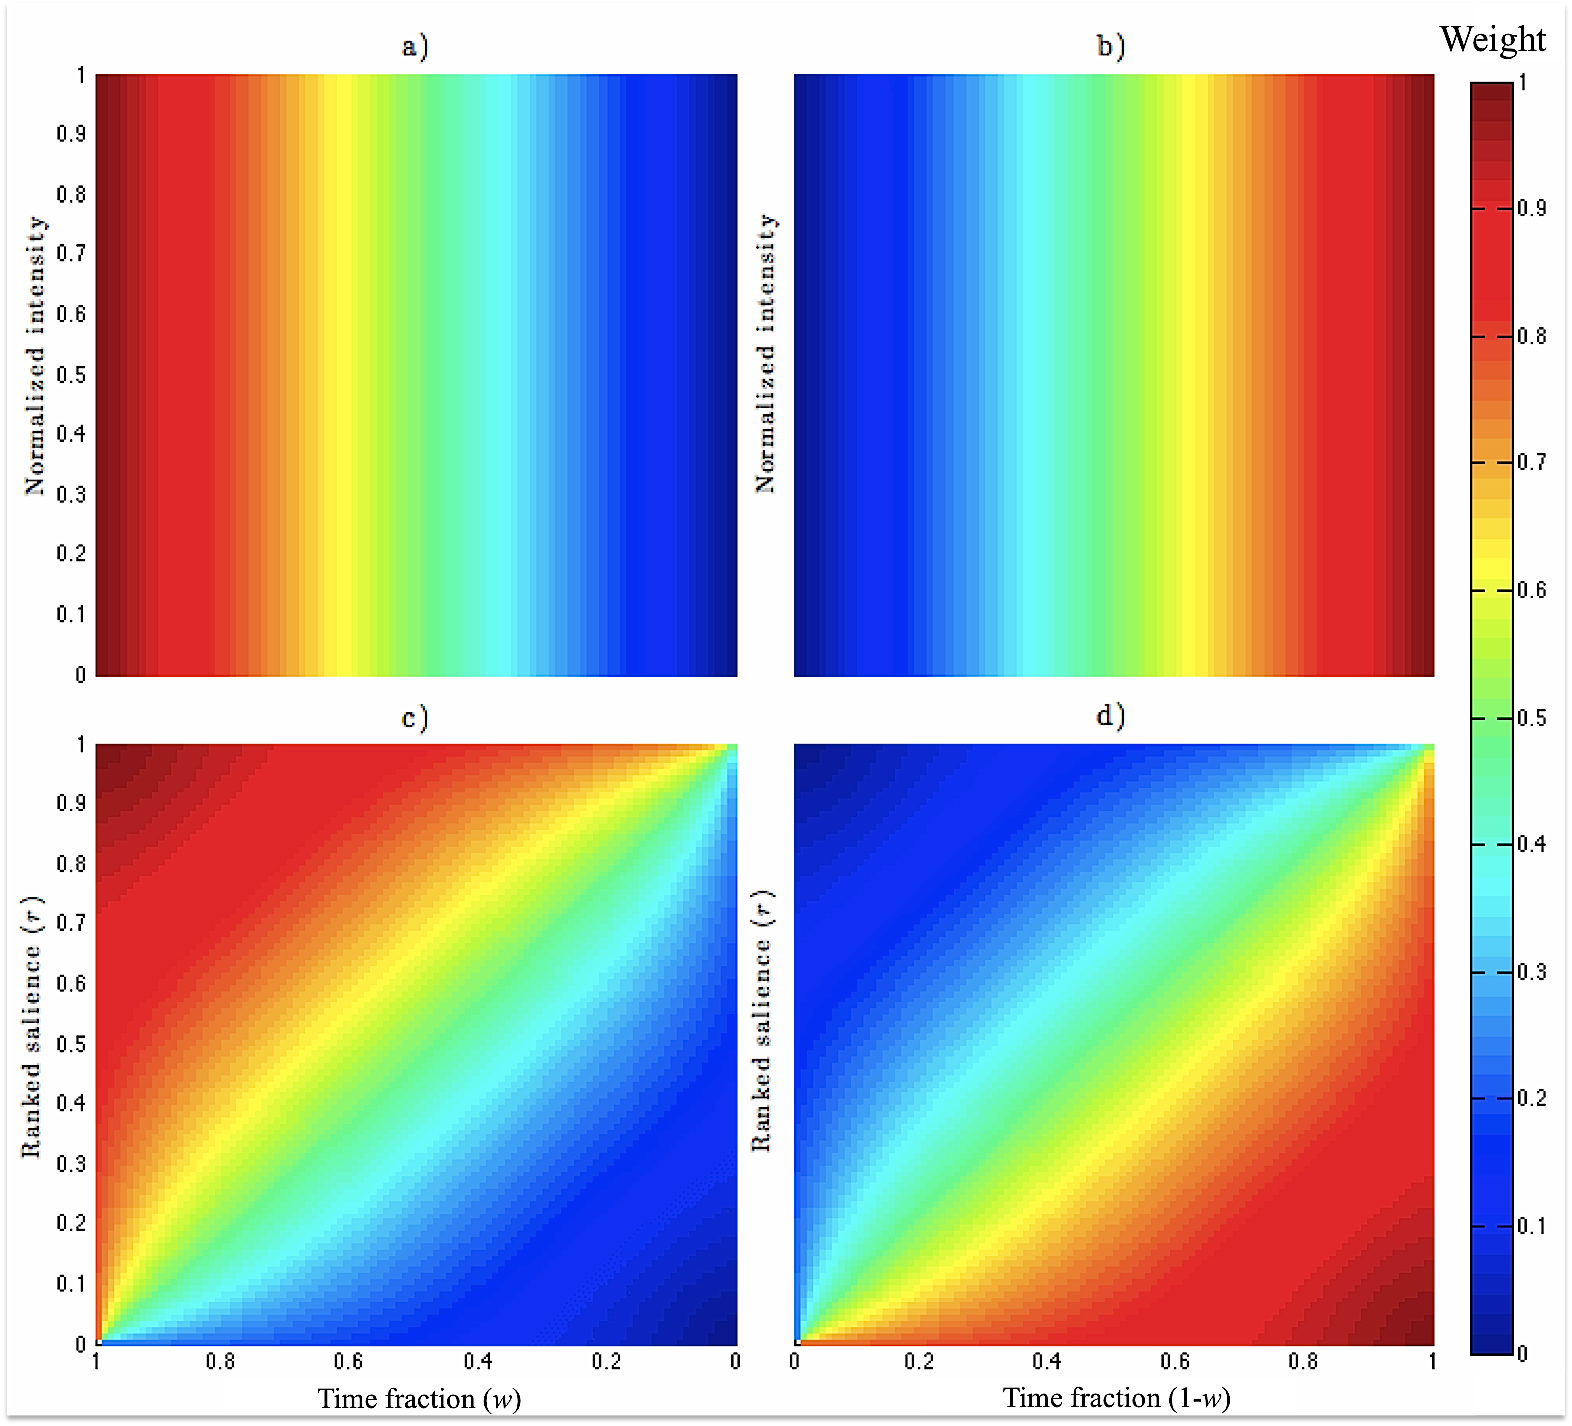
\includegraphics[width=39pc,angle=0]{f1.pdf}
%\caption{a) Linear cross-dissolve weights for extrapolation. Note that weights start at 1 regardless of intensity at 0 h and steadily decrease to 0 at maximum forecast length. 
%b) Linear cross-dissolve weights for HRRR model. Note that weights start at 0 regardless of intensity at 0 h and steadily increase to 1 at maximum forecast length. 
%c) Salient cross-dissolve weights ($w_{s}$) for extrapolation. Note that the weight of high intensity pixels (ranked saliency, $r$=$y$ axis, close to 1.0) remain high throughout the time period where low intensity pixels are dampened more quickly  
%d) Salient cross-dissolve weights ($w_{s}$) for model. The high intensity pixels ($r$ is close to 0) remain high throughout the time period.
%}
%\label{f1}
%\end{center}
%\end{figure}

%---------------------------------------------------------------------------------------------------------

\bibliographystyle{ametsoc}
\newpage
\bibliography{yunsung}

\end{document}
